%---------------------------------------------------------------
%	UNIVERSIDADE FEDERAL DE UBERLÂNDIA
%	Faculdade de Engenharia Elétrica
%	Programa de Pós-Graduação em Engenharia Elétrica
%	Programa de Pós-Graduação em Engenharia Biomédica
%	Laboratório de Engenharia Biomédica
%	Dissertação de Mestrado
%	Capítulo 1: Introdução
%---------------------------------------------------------------
\section{Introdução}
\label{cap:introducao}
\subsection{Circuitos magnéticos e materias magnéticos}
Os transformadores e máquinas elétricas, de forma geral, utilizam material ferromagnético para direcionar e dar forma a campos magnéticos, os quais atuam como meio de transferência e conversão de energia. Um circuito magnético consiste em uma estrutura que, em sua maior parte, é composto por material magnético de permeabilidade elevada. A presença de um material de alta permeabilidade tende a fazer com que o fluxo mangético seja confinado aos caminhos delimitados pela estrutura, do mesmo modo que, em um circuito elétrico, as correntes são confinadas aos condutores \cite{Fitzgerald2008}. A figura \ref{circ_mag_simp} apresenta um exemplo simplificado de um circuito magnético. Nesse caso, assume-se que o núcleo seja composto de material magnético cuja permeabilidade é muito maior que a do ar (\textmu >> \textmu\textsubscript{o}). A fonte do campo magnético do núcleo é o produto entre o número de espiras (N) e a corrente (i), expressa em ampères-espira (Ae). A força magnetomotriz (FMM) que atua no circuito magnético é dada pelo produto Ni. Diferente do circuito apresentado aqui, transformadores e a maioria das máquinas rotativas possuem no mínimo dois enrolamentos, de forma que Ni deve ser ajustado pela soma algébrica dos ampères-espiras de todos os enrolamentos. O fluxo magnético que atravessa uma superfície S é a integral de superfície da componente normal de B expressa pela equação \ref{fluxmag}.
\begin{equation}
\label{fluxmag}
\phi = \int_{S} B * da [Wb]
\end{equation}
A equação \ref{fluxmag} pode ser reduzida a uma equação escalar simples, uma vez que é considerado que a densidade de fluxo magnético é uniforme em uma seção reta de um circuito magnético.
\begin{equation}
\phi_{c} = B_{c} A_{c}
\end{equation}
Onde:
\begin{itemize}
\item \textphi\textsubscript{c} = fluxo no núcleo
\item B\textsubscript{c} = densidade de fluxo no núcleo
\item A\textsubscript{c} = área da seção reta do núcleo
\end{itemize}

A relação entra a força magnetomotriz que atua ao longo de qualquer segmento de um circuito magnético e o campo magnético naquele circuito pode ser calculada como:
\begin{equation}
\label{fmmeq}
FMM = Ni = \oint H dl
\end{equation}
As dimensões do núcleo são tais que o comprimento do caminho de qualquer linha de fluxo é aproximadamente igual ao comprimento médio do núcleo l\textsubscript{c}. A integral de linha torna-se o produto escalar H\textsubscript{c} I\textsubscript{c} do módulo de H vezes o comprimento médico l\textsubscript{c} do caminho do fluxo. A equação \ref{fmmeq} pode ser reescrita da seguinte forma:
\begin{equation}
FMM = Ni = H_{c}l_{c}
\end{equation}
Onde H\textsubscript{c} é o módulo médio de H no núcleo.
A relação entre a intensidade de campo magnético (H) e a densidade de fluxo magnético (B) é uma propriedade do material em que se encontra o campo magnético. É comum supor uma relação linear entre as duas variáveis, expressa por:
\begin{equation}
B = \mu H
\end{equation}
Onde \textmu \ é a permeabilidade magnética do material.
\begin{figure}[H]
\centering
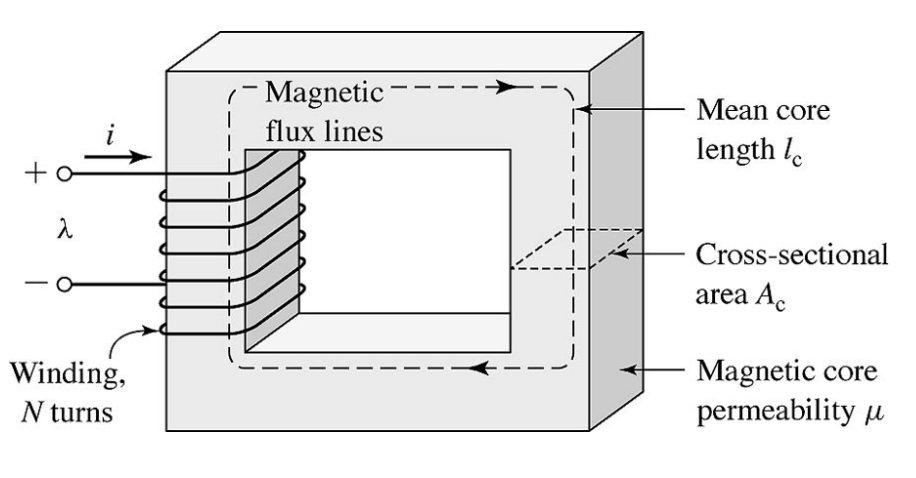
\includegraphics[scale=0.55]{img/assig1/simple_magnetic_circuit.png}
\caption[Circuito magnético simplificado]{Circuito magnético simplificado}
\label{circ_mag_simp}
\end{figure}
A tabela \ref{comp_ele_mag} apresenta uma analogia entre as variáveis dos circuitos elétricos e magnéticos.
\begin{table}[H]
\centering
\caption{Comparação entre variáveis dos circuitos elétricos e magnéticos}
\label{comp_ele_mag}
\begin{tabular}{lclc}
\hline
\multicolumn{2}{l}{\textbf{Circuito elétrico}} & \multicolumn{2}{l}{\textbf{Circuito magnético}} \\ \hline
Grandeza                          &     & Grandeza                           &     \\ \hline
Corrente                          & I          & Fluxo magnético                    & \straightphi        \\
Densidade de corrente             & J          & Densidade de fluxo magnético       & B          \\
Força eletromotriz                & V          & Força magnetomotriz                & FMM         \\
Intensidade de campo elétrico     & E          & Intensidade de campo magnético     & H          \\
Condutividade elétrica            & \textsigma      & Permeabilidade magnética           & \textmu         \\
Resistência                       & R          & Relutância                         & R'          \\ \hline
\end{tabular}
\end{table}
